\documentclass[11pt]{article}
\usepackage[letterpaper,margin=1in]{geometry}
\usepackage{fontspec}
\setmainfont{Latin Modern Roman}
\setsansfont{Latin Modern Sans}
\setmonofont{DejaVu Sans Mono}[Scale=.78]
\usepackage{amsmath,amssymb,amsthm,mathtools,microtype,booktabs,array,tabularx,enumitem,xcolor,needspace}
\usepackage{cite}
\usepackage{tikz,pgfplots}
\usetikzlibrary{arrows.meta,positioning,calc,shapes.geometric,fit,backgrounds}
\pgfplotsset{compat=1.18}
\usepackage[unicode,colorlinks=true,linkcolor=blue!40!black,citecolor=blue!40!black,urlcolor=blue!40!black]{hyperref}
\mathchardef\UrlBigBreakPenalty=10000
\hypersetup{pdftitle={Exact Sampling from Neural Networks: Conference Version},pdfauthor={Samuel Mausberg}}
\newtheorem{theorem}{Theorem}[section]
\newtheorem{lemma}[theorem]{Lemma}
\newtheorem{proposition}[theorem]{Proposition}
\newtheorem{corollary}[theorem]{Corollary}
\theoremstyle{definition}\newtheorem{definition}[theorem]{Definition}
\theoremstyle{remark}\newtheorem{remark}[theorem]{Remark}
\newcommand{\E}{\mathbb E}\newcommand{\PP}{\mathbb P}
\newcommand{\R}{\mathbb R}\newcommand{\N}{\mathbb N}
\newcommand{\sgn}{\operatorname{sgn}}\newcommand{\poly}{\operatorname{poly}}\newcommand{\Bern}{\operatorname{Bern}}
\newcommand{\Pois}{\operatorname{Pois}}\newcommand{\sech}{\operatorname{sech}}
\DeclareMathOperator{\rank}{rank}\DeclareMathOperator{\TV}{TV}
\newcolumntype{Y}{>{\raggedright\arraybackslash}X}
\setlist{nosep,leftmargin=1.5em}
\setlength{\emergencystretch}{2em}\setlength{\parskip}{2pt}
\numberwithin{equation}{section}
\title{Exact Sampling from Neural Networks:\\Depth, Attention, and Decoding}
\author{Samuel Mausberg\\{\normalsize Independent Researcher}}
\date{8 October 2026\quad\textit{Conference version}}
\begin{document}\maketitle
\begin{abstract}
A random output can require less information than the value of a
function. We study this difference for neural networks, counting input
probes, random bits, arithmetic, and precision refinement. A single
bounded tanh row admits an exact sample using a constant expected
number of input coordinates. When every absolute row sum is at most one,
the zero-bias worst-case query cost lies between the square root of
depth and depth. The sharp square-root law holds at every fixed
first-layer rank and for a bounded column envelope, with sufficient
input size.

The main theorem concerns decoding after prefill. If each head's keys
lie in a common affine space of fixed dimension, an exact decoder with
positive RMSNorm stabilizers can construct and append its own keys and
values in expected time polynomial in model size and polylogarithmic in
context length. The proof maintains finite Taylor moments and prepares
higher precision in the background. Rare complete refinements preserve
the exact original autoregressive law. The decoder's polynomial degree grows
with rank. These bounds give no useful speed prediction at the large
ranks of ordinary models. Without a context index, standard score
scaling can force linear search; arbitrary growing-dimensional indexed
queries also face a conditional hardness barrier. We give checkpoint
quantities that determine which positive bound can be applied, and
state the unrestricted zero-bias exponent as the main open problem.
\end{abstract}

\section{Why one sample can be cheaper}

Computing an average of $n$ arbitrary signs requires reading every
sign. Sampling one uniform coordinate gives a sign with that average
as its expectation. The same distinction persists through some
nonlinear computations. It does not follow by independently replacing
every activation with an unbiased random estimate: a nonlinear map of
that estimate generally has a different expectation.

We follow the information available to a decoder. A fresh input permits
only weight preprocessing. A supplied cache permits an index over keys
and values. A complete decoder must also create the next cache records,
and must do so as precision increases. These are different algorithmic
problems. An input-probe lower bound before prefill does not give a
query lower bound after an index has read the context.

This version gives complete proofs of the maintained decoder theorem
and its finite-cache building blocks. The full version~\cite{mausbergfull2026}
contains the depth-dependent factory and lower-bound proofs, the sharp
critical subclass theorems, and the additive-residual laws. Those results locate
the decoder theorem within the broader sampling question. The dominant
restriction is geometric: a rank bound independent of width is needed
for a uniform polynomial in width. Fixing every parameter of a full-rank
model also gives a formal polylogarithmic context bound, but its exponent
can be enormous. This is an asymptotic existence result, with no claimed
checkpoint speedup.

\section{Model and principal theorem}
\label{sec:conf-model}

A dyadic number is an integer divided by a power of two. All fixed
parameters have binary encoding length at most $b$, with denominators
dividing $2^b$. Let $n$ be residual width, $D$ the number of blocks,
$V$ the vocabulary size, $T_0\ge1$ the prompt length, and $T$ the current
context length. We use one head of dimension $n$. Rectangular
heads are treated in the full version~\cite{mausbergfull2026}.
The norm of a matrix is its maximum absolute row sum,
$s(W)=\max_i\sum_j|W_{ij}|$. Embeddings, affine bias coordinates, and
all matrix row norms are bounded by $s\ge1$.
Table~\ref{tab:conf-notation} collects the notation.

For $\varepsilon>0$, define the unscaled normalization
\[
 N_\varepsilon(h)=\frac{h}{\sqrt{\varepsilon+\|h\|_2^2/n}}.
\]
Each block computes affine queries $q_t$, keys $k_t$, and values $v_t$
from $N_\varepsilon(h_t)$ and uses the causal attention mean
\begin{equation}
 a_{tj}=\frac\beta n\langle q_t,k_j\rangle,\qquad
 u_t=\frac{\sum_{j\le t}e^{a_{tj}}v_j}{\sum_{j\le t}e^{a_{tj}}}.
 \label{eq:conf-attention}
\end{equation}
An affine map of $u_t$ is added to $h_t$. A second normalization,
affine map, and coordinatewise tanh supply the other additive update.
Either update may be multiplied by a fixed coefficient in $[0,1]$;
convex residual mixtures are allowed as well. An affine head gives
$V$ logits $z_i$, followed by probabilities
$p_i=e^{z_i}/\sum_j e^{z_j}$. No bounded-logit promise is needed.
All stabilizers satisfy $\varepsilon\ge2^{-b}$. The temperature is a
nonnegative dyadic number or the exact algebraic number $\beta=\sqrt n$.
Each affine key map is fixed across positions and its linear part has
rank at most $r$. Thus all keys of one layer lie in one known affine
space, including keys not yet generated. A separate rank bound at each
position would not suffice.

\begin{theorem}[An exact maintained decoder]
\label{thm:conf-decoder}
For every fixed $r$, the preceding model has a uniform exact
sampler and a constructive polynomial $F_r$ such that prefill costs
\[
 T_0F_r(n,D,V,b,s,\beta,\log(T_0+2)),
\]
and the conditional expected bit work of each subsequent token is at most
\[
 F_r(n,D,V,b,s,\beta,\log(T+2)).
\]
The cost includes constructing and appending its neural keys and values,
all random bits, and every precision refinement. The conditional law is
the original model's law for every realized token history. At standard
scaling and polynomially bounded $D,V,b,s$, the cost is
$\poly_r(n,\log T)$. The degree depends on $r$.
\end{theorem}

The theorem concerns the real functions defined by the stored finite
parameters. It does not assert equality with a particular floating-point
implementation. It includes pre-norm additive residuals and a positive
normalization stabilizer; neither a small row norm nor contraction is
needed. Large norms instead increase the moment degree and working
precision. The proof occupies Sections~\ref{sec:conf-moments}--\ref{sec:conf-replay}.
Figure~\ref{fig:assumptions-to-costs} shows what each kind of
preprocessing changes.

\begin{table}[t]\centering\small
\begin{tabularx}{\textwidth}{@{}p{.18\textwidth}Y p{.18\textwidth}Y@{}}
\toprule
Quantity & Meaning & Quantity & Meaning\\\midrule
$n,D,V$ & Width, depth, vocabulary & $T,T_0$ & Current and prompt lengths\\
$b,B$ & Parameter and total bit scales & $r$ & Common affine key dimension\\
$Q_{\max},K$ & Query and key coordinate bounds & $\beta$ & Score temperature\\
$A_{\rm coin},H$ & Score-coin amplitude; moment coefficient bound & $P,m,N_m$ & Working bits, Taylor degree, feature count\\
$\varepsilon,\lambda$ & Stabilizer; certified squared-denominator floor & $Q$ & Distinct fresh-input probes\\
\bottomrule
\end{tabularx}
\caption{Notation. $B=16+b+\lceil\log_2(T+n+D+V+r+2)\rceil$;
fixed rational chart lengths are included when used.}
\label{tab:conf-notation}
\end{table}

\begin{figure}[t]
\centering
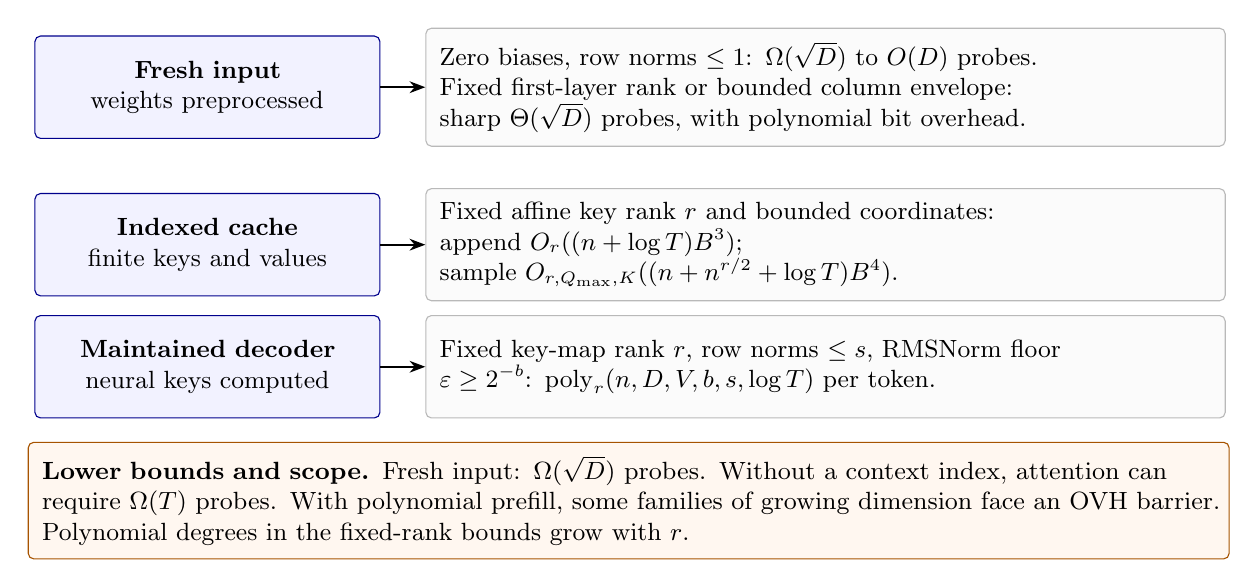
\begin{tikzpicture}[
 >=Stealth,font=\small,
 access/.style={draw=blue!55!black,fill=blue!5,rounded corners=2pt,
                text width=4.1cm,minimum height=13mm,align=center,
                inner sep=4pt},
 result/.style={draw=gray!55,fill=gray!3,rounded corners=2pt,
                text width=9.8cm,minimum height=13mm,align=left,
                inner sep=5pt},
 edge/.style={->,semithick}]
 \node[access] (fresh) at (0,0)
   {\textbf{\mbox{Fresh input}}\\\mbox{weights preprocessed}};
 \node[result] (freshcost) at (7.85,0)
   {Zero biases, row norms $\le1$: $\Omega(\sqrt D)$ to $O(D)$ probes.\\
    Fixed first-layer rank or bounded column envelope:\\
    sharp $\Theta(\sqrt D)$ probes, with polynomial bit overhead.};
 \node[access] (cache) at (0,-2.0)
   {\textbf{\mbox{Indexed cache}}\\\mbox{finite keys and values}};
 \node[result] (cachecost) at (7.85,-2.0)
   {Fixed affine key rank $r$ and bounded coordinates:\\
    append $O_r((n+\log T)B^3)$;\\
    sample $O_{r,Q_{\max},K}((n+n^{r/2}+\log T)B^4)$.};
 \node[access] (neural) at (0,-3.55)
   {\textbf{\mbox{Maintained decoder}}\\\mbox{neural keys computed}};
 \node[result] (neuralcost) at (7.85,-3.55)
   {Fixed key-map rank $r$, row norms $\le s$, RMSNorm floor\\
    $\varepsilon\ge2^{-b}$: $\operatorname{poly}_r(n,D,V,b,s,\log T)$ per token.};
 \draw[edge] (fresh)--(freshcost);
 \draw[edge] (cache)--(cachecost);
 \draw[edge] (neural)--(neuralcost);
 \node[draw=orange!65!black,fill=orange!6,rounded corners=2pt,
       align=left,text width=14.9cm,inner sep=5pt]
       at (5.35,-5.25)
   {\textbf{Lower bounds and scope.}
    Fresh input: $\Omega(\sqrt D)$ probes. Without a context index,
    attention can require $\Omega(T)$ probes. With polynomial prefill,
    some families of growing dimension face an OVH barrier.
    Polynomial degrees in the fixed-rank bounds grow with $r$.};
\end{tikzpicture}
\caption{What preprocessing changes. The first row counts expected input
 probes; the other rows count expected bit work. Every law is exact.
 Here $n$ is width, $D$ depth, $T\ge2$ cache length, and $V$ vocabulary;
 $B$ includes parameter encodings and address bits. Attention uses
 $\beta=\sqrt n$. Finite-cache coordinate bounds $Q_{\max},K$ are fixed;
 the decoder incorporates them through $n,s$. Fresh-input preprocessing
 uses $D=\lceil\log_2n\rceil$ and
 $\lceil\log_2(D+1)\rceil\le b=O(\log n)$, where $b$ is
 parameter precision. Its column envelope is $\sum_j\max_i|w_{1,ij}|$.
 OVH is the randomized Orthogonal Vectors Hypothesis.}
\label{fig:assumptions-to-costs}
\end{figure}


\section{A scalar example and the preprocessing boundary}
\label{sec:conf-scalar}

A sign interface for $u/R\in[-1,1]$ returns independent signs of that
mean. Products of independent signs multiply means; random selection
among interfaces takes a convex combination. A Bernoulli factory uses
such requests to transform an unknown mean. These principles are
classical~\cite{gaines1967,nacuperes2005,holtz2011,dughmi2017}.

\begin{proposition}[One bounded tanh row]
\label{prop:conf-row}
Let $u=c+\sum_jw_jx_j$, where $x_j\in\{-1,1\}$, $|c|\le1$,
and $\sum_j|w_j|\le1$. After $O(nB^2)$ weight preprocessing, one can
return a sign of mean $\tanh u$ using $O(1)$ expected input requests
and $O(B^4)$ expected bit work.
\end{proposition}
\paragraph{Proof idea.}
A random coordinate supplies the linear mean. An exponential acceptance
race then selects between the two signs with the logistic probabilities.
\begin{proof}
Put $A=|c|+\sum_j|w_j|\le2$. If $A=0$, return a fair sign.
Otherwise a weighted choice among $\sgn(c)$ and $\sgn(w_j)x_j$
returns a sign of mean $u/A$. Integer cumulative weights implement this
choice exactly in $O(B^2)$ expected bit work after preprocessing.
Propose $Y=\pm1$ uniformly and draw $N\sim\Pois(2A)$. Accept if all
$N$ independent bits of bias $(1+Yu/A)/2$ are one. The Poisson generating
function gives acceptance $e^{Yu-A}$. Hence the accepted sign has mean
\[
 \frac{e^u-e^{-u}}{e^u+e^{-u}}=\tanh u.
\]
A trial succeeds with probability $e^{-A}\cosh u\ge e^{-A}$.
Its expected source count is at most $2A$, so renewal gives at most
$2Ae^A\le4e^2$ requests. Here is a finite-bit Poisson implementation, within the classical
Buffon-machine framework~\cite{flajolet2011buffon}. For $\lambda=2A\le4$,
propose $K\ge0$ with probability $2^{-(K+1)}$ using fair bits, and accept
with probability $e^{-\lambda}(2\lambda)^K/(128K!)$. This is at most
$e^4/128<1$. Its accepted mass is
$e^{-\lambda}\lambda^K/(256K!)$, so each trial succeeds with probability
$1/256$ and the accepted $K$ is Poisson. The rational factor is below
$e^8/128<52$ and has $O(K[B+\log(K+2)])$ bits. A finite exponential
series on $[0,4]$ gives certified acceptance intervals with polynomial
work. Geometric proposal and uniform-comparison tails have all fixed
moments; summing their polynomial costs gives $O(B^4)$ expected work.
Thus neither the Poisson draw nor the acceptance test uses a real oracle.
\end{proof}

For attention, suppose $|a_j|\le A_{\rm coin}$ and a sign of mean
$a_j/A_{\rm coin}$ is available. The Poisson test accepts a uniform
proposal $j$ with probability $e^{a_j-A_{\rm coin}}$, giving the
exact attention law.

The expected predecessor count, including
a fresh value sign, is at most $2e^{2A_{\rm coin}}-1$ when each score
test uses two predecessor signs; the stopped-test calculation is given
in the full version. A bounded score range therefore can remove the
linear context factor before prefill. Standard scaling alone cannot.

Here is the search obstruction in its simplest form. At a fresh
all-negative sign context, give position $j$ score $Ax_j$ and value
$x_j$. Changing only coordinate $i$ makes its positive attention mass
\[
 \frac{e^{2A}}{T-1+e^{2A}}.
\]
Couple an exact sampler's random tapes on the two inputs. Their outputs
can differ only after coordinate $i$ is read, so the probability of that
read is at least the total-variation distance of the target laws.
Summing over $i$ forces $\Omega(\min\{T,e^{2A}\})$ probes. A bounded
tanh and binary-softmax head preserve the gap up to an absolute constant;
a convex residual gate multiplies it by its weight $\alpha$.
The matching one-block family has cost
$\Theta(1+\alpha\min\{T,e^{2\beta s^2}\})$~\cite{mausbergfull2026}.
Thus $2\sqrt n\,s^2\ge\log T$ can force linear context search. An index
built from those signs is already different on the two inputs, so this
coupling does not yield an online lower bound after prefill.

\section{An index for supplied finite keys}
\label{sec:conf-grid}

A bounded coordinate chart turns fixed affine dimension into a finite
number of score cells. The index in this section returns an attention
index; Section~\ref{sec:conf-moments} instead maintains attention means
for the complete decoder.

\begin{lemma}[Bounded rational coordinates]
\label{lem:conf-chart}
For an $n\times d$ full-column-rank dyadic matrix $U$, with $d\le r$
and $b$-bit entries, one can find $d$ row indices $I$ so that
$A=U(U_I)^{-1}$ satisfies $A_I=I_d$ and $|A_{ij}|\le2$.
The work is $O_r(nB^3)$ and all chart coefficients have $O_r(B)$ bits.
\end{lemma}
\paragraph{Proof idea.}
A large reconstruction coefficient identifies a row replacement that
more than doubles a nonzero integer determinant.
\begin{proof}
Clear the common dyadic denominator and start with any nonsingular row
minor of the resulting integer matrix $E$. If $|[E(E_I)^{-1}]_{ij}|>2$,
replace selected row $j$ by row $i$. Determinant multilinearity multiplies
the determinant's absolute value by that coefficient. The new row is
distinct because selected rows have identity coefficients. A nonzero
integer minor has magnitude at least one; every minor has magnitude at
most $d!\|E\|_{\max}^d$. Only $O_r(B)$ replacements occur. Each stage
uses $O_r(nB^2)$ schoolbook bit work. Cramer's rule gives the stated
coefficient lengths and a common determinant denominator. This is the
standard maximum-volume argument~\cite{mikhalev2018maxvol}.
\end{proof}

\begin{theorem}[Appendable finite cache]
\label{thm:conf-grid}
Fix $r$, dyadic bounds $K,Q_{\max}>0$, and $\beta\ge0$ dyadic or
$\sqrt n$. A stream of $b$-bit keys in $[-K,K]^n$, whose every prefix
has affine dimension at most $r$, admits an exact attention-index
sampler for explicitly supplied dyadic queries in $[-Q_{\max},Q_{\max}]^n$.
Queries occur at nonempty prefixes. All scalar encodings of keys, queries,
coordinate bounds, and dyadic temperature have at most $b$ bits. With
$\beta\le\bar\beta\le2\beta$ dyadic when $\beta>0$, its append cost
is $O_r((n+\log(T+2))B^3)$ and its expected query cost is
\[
 O_r((n+M_T+\log(T+2))B^4),\qquad
 M_T\le\min\{T,(r+1)(5+32r\bar\beta Q_{\max}K)^r\}.
\]
It stores $O_r((T+1)nB)$ bits. No append scans previous records.
\end{theorem}
\paragraph{Proof idea.}
Keep each old chart when the span grows. Within a chart, a grid makes
one score representative a constant-factor envelope for its whole cell.
\begin{proof}
The case $\beta=0$ is uniform sampling. Otherwise fix the first key $c$.
Maintain a basis of differences $k_j-c$. At each increase of rank start
a new chart from Lemma~\ref{lem:conf-chart}, and retain every earlier
chart and its records. At most $r+1$ charts are ever used. Within one
chart, $k=c_0+Ak_I$, where $c_0=c-Ac_I$ and $k_I\in[-K,K]^d$.
A query's coordinate coefficients obey $|(q^TA)_i|\le2nQ_{\max}$.
Use grid width $\Delta=K2^{-h}$, with
$h=\lceil\log_2\max(1,8r\bar\beta Q_{\max}K)\rceil$.
Two keys in a cell have score difference below
$2\beta rQ_{\max}\Delta\le1/4$. There are at most
$(5+32r\bar\beta Q_{\max}K)^d$ cells in a chart.

Store occupied cells in a balanced tree and their member identifiers in
binary append trees. Membership in the current span is tested by the
exact equality $k-c=A(k_I-c_I)$. A failed test creates the next chart;
all old records stay in place. An insertion takes the stated work,
including a chart change, and identifier storage is linear in $T$.

At query time compute $q^TA$ and $\langle q,c_0\rangle$ once per
chart. Let $a_C$ be each occupied cell's representative score and
$a_0=\max_Ca_C$. Put $w_j=e^{a_j-a_0-1/4}$ and
$e_C=e^{a_C-a_0}$. Then $w_j\le e_C<2w_j$ in that cell, while
$Z=\sum_jw_j>1/2$. Set $p=\lceil\log_2(64T)\rceil$ and compute
positive dyadic upper bounds
\[
 e_C\le u_C\le e_C+3\,2^{-p},\qquad u_C\ge2^{-p}.
\]
Enclose $e_C$ to width $2^{-p-2}$, round the upper endpoint up to the
$2^{-p}$ grid, and add one grid unit. The envelope mass satisfies
$Z\le W=\sum_C|C|u_C<2Z+3/64<(17/8)Z$.
Choose a cell with weight $|C|u_C$, then a uniform member $j$, and
accept with probability $w_j/u_C$. The accepted mass is exactly
$w_j/W$, so the result has the target law and the expected number of
proposals is below $17/8$.

All representative comparisons are rational before multiplication by
$\beta/n$. At standard scaling an exponent is a rational plus a
rational multiple of $1/\sqrt n$. Bisection encloses that square root.
For a nonpositive exponent, values below $-(p+2)\log2$ may be enclosed
by $[0,2^{-p-2}]$; on the remaining interval the exponential Taylor
series with range reduction costs a fixed polynomial in $B+p$.
Near the cutoff either safe enclosure can be used after a constant
overlap, so no exact equality test is needed. Since $u_C\ge2^{-p}$,
$t+O(p)$ exponential bits suffice for acceptance at precision $t$.
The probability of an undecided uniform comparison is $O(2^{-t})$.
Summing that geometric tail against the polynomial refinement work
gives $O(B^4)$ expected work per proposal. Exact integer cumulative
weights give the cell choice. One projection per chart and one initial
enclosure per occupied cell prove the query bound. All statements
condition on the supplied records and query, so adaptivity is allowed.
\end{proof}

\paragraph{Worked example: two repeated keys.}
Suppose the cache contains $N_+$ copies of $\mathbf1$ with value $+1$
and $N_-$ copies of $-\mathbf1$ with value $-1$. Put
$T=N_++N_-$ and $M=n^{-1}\sum_iq_i$. Its attention mean is
\[
 u(q)=\frac{N_+e^{\beta M}-N_-e^{-\beta M}}
            {N_+e^{\beta M}+N_-e^{-\beta M}}.
\]
The index has at most three occupied cells, at most two in the second
chart. An append changes one count;
a fresh query requires its scalar projection and two score weights.
Theorem~\ref{thm:conf-grid} gives expected query cost
\mbox{$O((n+\log(T+2))B^4)$}, even at $\beta=\sqrt n$.
For a balanced cache, $u(q)=\tanh(\beta M)$. Prefill removes the
context-length scan while retaining the work needed to read a fresh query.

\section{Finite moments with certified error}
\label{sec:conf-moments}

The grid uses finite supplied keys. Neural keys are usually irrational,
and their required accuracy changes over time. For the complete decoder
we maintain a polynomial evaluator at each chosen precision. Taylor
feature sums for causal attention are established representations
\cite{katharopoulos2020linear,heinsen2026taylor}. The following lemma
records the finite arithmetic and error guarantee that exact sampling
needs.

\begin{lemma}[A finite moment evaluator]
\label{lem:conf-moments}
Let $z_j\in[-1,1]^r$ and $v_j\in[-1,1]^a$ lie on a common dyadic
grid $2^{-P}$. For $\|t\|_1\le H$, $H\ge1$ an integer, an appendable
index encloses every coordinate of
\[
 A(t)=\frac{\sum_{j\le T}e^{\langle t,z_j\rangle}v_j}
              {\sum_{j\le T}e^{\langle t,z_j\rangle}}
\]
to width $2^{-p}$. Its finite arithmetic is polynomial in
$a,H,P,p$, rational input lengths, $\log(T+2)$, and, for coefficients
with $1/\sqrt n$, $\log(n+2)$, at fixed $r$.
The coefficients of $t$ may be rational with a common denominator,
or rational multiples of $1/\sqrt n$. The index has
$(a+1)N_m$ integer counters, where
\begin{equation}
 m=\lceil8(p+3H+7)\rceil,\qquad N_m=\binom{m+r}{r}.
 \label{eq:conf-features}
\end{equation}
\end{lemma}
\paragraph{Proof idea.}
Store sums of every monomial up to degree $m$. The sums are exact;
only a finite Taylor truncation and the final certified division need
error allowances.
\begin{proof}
Put $q=p+2H+6$ and $E_m(x)=\sum_{d=0}^m x^d/d!$.
The factorial inequality $N!\ge(N/e)^N$, obtained by integrating
$\log x$ below its sum, gives
\[
 \sup_{|x|\le H}|e^x-E_m(x)|
 \le e^H H^{m+1}/(m+1)!\le2^{2H-m-1}\le2^{-q}.
\]
Here $m+1\ge8H$ and $e<4$. Store
$S_\nu=\sum_jz_j^\nu$ and $M_{\nu,i}=\sum_jz_j^\nu v_{j,i}$
for $|\nu|\le m$ as integer numerators over $2^{P(m+1)}$.
Each numerator has $O(P(m+1)+\log(T+2))$ bits. Insertion adds exact
integer increments, so the index acquires no rounding error with age.
The identity
\[
 E_m(\langle t,z\rangle)=\sum_{|\nu|\le m}\frac{t^\nu z^\nu}{\nu!}
\]
evaluates the truncated numerator and denominator from the counters.
If $d_t$ is a common rational denominator for $t$, the coefficient
denominators divide $d_t^m m!$, since $\nu!$ divides $m!$.
All intermediate integer lengths are polynomial in the parameters.

Divide both sums by $T$. The true denominator $Z$ obeys $Z\ge e^{-H}$,
the numerator satisfies $|N_i|\le Z$, and each Taylor error is at most
$\delta=2^{-q}$. Thus the truncated denominator is positive and
\[
 \left|\frac{\widetilde N_i}{\widetilde Z}-\frac{N_i}{Z}\right|
 \le\frac{2\delta}{Z-\delta}\le4\delta e^H\le2^{-p-4}.
\]
Rational division to width $2^{-p-2}$, enlarged by this error, gives
the required interval. If $t_i=c_i/\sqrt n$, split monomials by parity
of $|\nu|$: each sum is $A+B/\sqrt n$ with rational $A,B$.
A common denominator divides
$d_c^m n^{\lfloor m/2\rfloor}m!$. Certified square-root bisection and
the lower bound $\widetilde Z\ge e^{-H}/2$ give the ratio with only
polynomial additional precision. This treats $\sqrt n$ exactly.
\end{proof}

\section{Errors propagate through depth}
\label{sec:conf-stability}

The maintained evaluator must enclose the network on the actual token
history. It cannot treat independently rounded keys as exact model
activations. We next construct one deterministic evaluator for every
requested precision.

\begin{lemma}[Uniform prefix evaluation]
\label{lem:conf-stability}
For the model of Theorem~\ref{thm:conf-decoder}, all next-token
cumulative probabilities can be enclosed to width $2^{-p}$ by a
maintained causal evaluator. Its per-token work is polynomial at fixed
$r$ in $n,D,V,b,s,\beta,p,\log(T+2)$. One may use working precision
\begin{equation}
 P=p+O\bigl((D+1)[b+\log(n+s+\beta+2)]+\log(D+V+2)\bigr).
 \label{eq:conf-P}
\end{equation}
A complete replay costs $T$ times the same polynomial.
\end{lemma}
\paragraph{Proof idea.}
Attention is uniformly Lipschitz in the largest error over the prefix.
Each layer reads the preceding layer's states, so errors accumulate with
depth. Exact moment sums prevent an additional recurrence in token count.
\begin{proof}
Write $p(a)$ for softmax. Its directional derivative is
$\dot p_j=p_j(\dot a_j-\sum_i p_i\dot a_i)$; hence
$\|p(a)-p(a')\|_1\le2\|a-a'\|_\infty$, independently of the
number of positions. If values are bounded by $K$, then
\begin{equation}
 \|A(a,v)-A(a',v')\|_\infty
 \le\|v-v'\|_\infty+2K\|a-a'\|_\infty.
 \label{eq:conf-attention-Lip}
\end{equation}
For queries and keys bounded by $K$, their score perturbation is at
most $\beta K(\delta_q+\delta_k)$, by subtracting one factor at a time.

Normalization satisfies $\|N_\varepsilon(h)\|_\infty\le\sqrt n$.
Its Jacobian has entries
$\delta_{ij}/\sqrt v-h_ih_j/(nv^{3/2})$, with
$v=\varepsilon+\|h\|_2^2/n$; the maximum absolute row sum is at most
$(1+\sqrt n)/\sqrt\varepsilon$. Choose a power of two
$K\ge s(\lceil\sqrt n\rceil+1)$ less than twice this bound.
All query, key, and value coordinates are then bounded by $K$.
Every affine map has Lipschitz constant at most $s$, and tanh at most
one. Residual addition, the affine head, and cumulative softmax have
polynomial Lipschitz bounds. Thus the whole prefix computation has
$J=O(D+1)$ stages on prefix arrays, each bounded by a common constant
$L_0\ge2$ with
$\log_2L_0=O(b+\log(n+s+\beta+2))$.

If local error at every stage is at most $\delta$, induction gives
final error at most $JL_0^J\delta$. Take
$P\ge p+\lceil\log_2(J+1)\rceil+J\lceil\log_2L_0\rceil+10$
and $\delta=2^{-P}$. A certified midpoint, followed by dyadic rounding,
implements a local approximation without deciding whether an unknown
real lies exactly on a grid boundary. Compute normalization to its
local error allowance, round it to the common grid, and clip to
$[-\lceil\sqrt n\rceil,\lceil\sqrt n\rceil]$. Compute
$\widetilde k=W_K\widetilde N+b_K$ \emph{exactly} on the resulting
grid. It remains in the affine key space. Independent rounding of key
coordinates would not preserve that promise. Compute the query and
value products similarly; round completed residual updates.

Apply Lemma~\ref{lem:conf-chart} to a column basis of $W_K$.
The common affine key space has coordinates $k=c_0+Ak_I$ with
$|A_{ij}|\le2$. Put $z_j=(k_j)_I/K$. The common score offset cancels,
and the remaining coefficients are
\[
 t=\frac{\beta K}{n}q^TA,\qquad \|t\|_1\le2r\beta K^2.
\]
Take an integer $H\ge\max(1,2r\beta K^2)$ and apply
Lemma~\ref{lem:conf-moments}, with the additional
$O(\log(K+2))$ local bits needed to rescale values. The chart has a
common determinant denominator of polynomial encoding length. Standard
scaling has exactly the coefficient form allowed by that lemma.
All moment counters are exact on the common grid for this precision.

Elementary finite series and bisection evaluate tanh and normalization
at dyadic arguments in polynomial time in the requested precision and
the stated range bounds. The residual range is at most
$s+D(sK+s+1)$; the affine logit range is consequently polynomial.
To evaluate softmax without an exponential range factor, first enclose
each logit to width $1/4$ and take $A$ as the largest upper endpoint.
Then $z_i-A\le0$ for all $i$, and some $z_i-A\ge-1/4$, so
$\sum_i e^{z_i-A}>1/2$. Intersect refined logit intervals with their original coarse enclosures;
the shifted upper endpoints remain nonpositive. Refining the negative
exponentials to $2^{-p-O(\log V)}$ and dividing certified intervals gives each cumulative
probability to width $2^{-p}$. No exact comparison between real logits
is required. All local error allowances can be enlarged by fixed guard
margins and propagated explicitly.

Process positions in increasing order. At position $t$ and each layer,
form its query, key, and value from the preceding-layer state, append
that record before the attention query, then complete the residual and
feedforward updates. This includes exactly $j\le t$. In the error
induction, take the maximum over every position in a prefix at each
layer. A previous token's error is never fed into the same layer's
residual state; attention reads the preceding layer. Equation
\eqref{eq:conf-attention-Lip} is uniform in prefix length, and exact
moment additions add no time error. This proves both the certificate
and its independence from a linear factor in $T$.
\end{proof}

For reference, elementary schoolbook arithmetic in the preceding
construction permits a deliberately coarse per-token bound
\begin{equation}
 \begin{aligned}
 &C_r(D+1)(n+V+1)^2(m+1)^{2r+4}L^4,\\
 &L=C_r\{m[P+b+\log(n+m+D+V+2)]+\log(T+2)+1\}.
 \end{aligned}
 \label{eq:conf-explicit}
\end{equation}
Here $m=O_r(1+\beta K^2+P)$, and chart lengths are included in $b$
up to the displayed rank-dependent constant. This formula makes the
rank dependence visible. The exact feature count~\eqref{eq:conf-features}
is more informative for a feasibility check than this loose upper bound.

\section{Exact decisions while precision grows}
\label{sec:conf-replay}

Interval sampling is classical~\cite{han1997interval,brassard2019remote}.
The issue for a growing neural cache is paying for increased precision.
The next lemma separates that scheduling question from the particular
network evaluator. Figure~\ref{fig:decoder-overview} outlines the schedule.

\begin{figure}[ht]
\centering
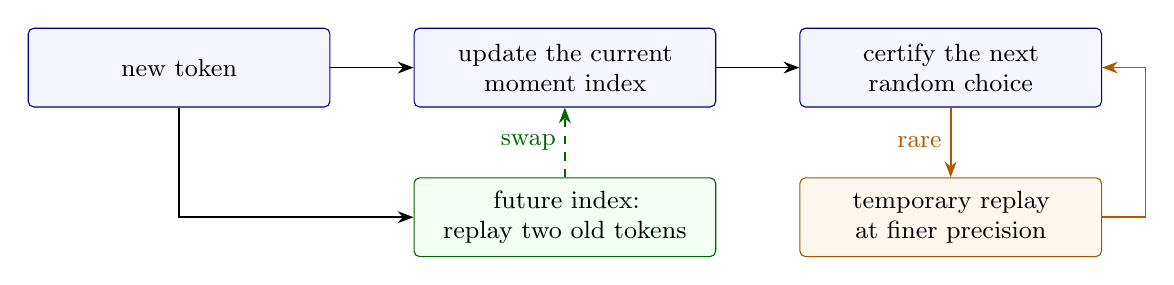
\begin{tikzpicture}[
 >=Stealth,font=\small,
 box/.style={draw=blue!55!black,fill=blue!4,rounded corners=2pt,
             minimum height=10mm,align=center,text width=3.55cm,
             inner sep=4pt},
 edge/.style={->,semithick}]
 \node[box] (token) at (0,0) {new token};
 \node[box] (current) at (4.9,0) {update the current\\moment index};
 \node[box] (sample) at (9.8,0) {certify the next\\random choice};
 \node[box,fill=green!5,draw=green!40!black] (future) at (4.9,-1.9)
   {future index:\\replay two old tokens};
 \node[box,fill=orange!7,draw=orange!65!black] (refine) at (9.8,-1.9)
   {temporary replay\\at finer precision};
 \draw[edge] (token)--(current);
 \draw[edge] (current)--(sample);
 \draw[edge] (token.south) |- (future.west);
 \draw[edge,green!40!black,dashed] (future.north)--
   node[left,inner sep=3pt] {swap}(current.south);
 \draw[edge,orange!70!black] (sample.south)--
   node[left,inner sep=3pt] {rare}(refine.north);
 \draw[edge,orange!70!black] (refine.east) -- ++(.55,0) |- (sample.east);
\end{tikzpicture}
\caption{Maintaining an exact decoder. A routine step evaluates the new
 token in the current index and replays at most two old tokens in a future index.
 The future index takes over when it catches up. If the random choice is
 too close to a probability boundary, a temporary finer replay resolves
 it. All three computations use the same discrete token history.}
\label{fig:decoder-overview}
\end{figure}


\Needspace{17\baselineskip}
\begin{lemma}[Maintained evaluation implies exact sampling]
\label{lem:conf-replay}
Suppose a deterministic causal evaluator at accuracy $p$ appends one
actual history token and returns certified cumulative probabilities of
width $2^{-p}$ in at most $G(p+\log(T+2))$ bit operations, where $G$
is a fixed polynomial with nonnegative coefficients. Include in $G$ the
work of comparing a $p$-bit uniform cell with those cumulative intervals;
a scan costs $O(V(p+1))$ bits and can be added to $G$ if needed. Suppose replaying
a length-$T$ history has cost at most $T G(p+\log(T+2))$.
Then an exact autoregressive sampler has polynomial expected per-token
work after a prompt pass. If $G(u)\le Au^k$ for $u\ge1$, put $S=1+\log(V+2)+\log(T+2)$. Its expected total bit
work is $O_k(AS^k+S)$. The expectation conditions on every realized history.
\end{lemma}
\paragraph{Proof idea.}
Use enough routine bits that an ambiguous output decision is rare even
after charging a complete replay. Prepare the next routine precision
by processing two historical tokens after each append.
\begin{proof}
At a power-of-two horizon $R$, use
$p_R=\lceil\log_2(64V(R+2)^3)\rceil$. Reveal the first $p_R$ bits
of a fresh uniform binary expansion $U$, giving a dyadic cell $[a,b]$.
Let $[\underline F_i,\overline F_i]$ enclose each cumulative boundary,
using exact $F_0=0,F_V=1$. Output $i$ if
$\overline F_{i-1}\le a$ and $b\le\underline F_i$. If undecided,
replay the actual history at accuracy $p_R+1$, reveal the next uniform
bit, and try again; continue similarly. Different replay intervals
need not be nested, because all contain the same exact boundaries.

If a precision-$p$ comparison is undecided, $U$ lies within $2^{1-p}$
of one of at most $V-1$ boundaries. Conditional on the history,
\begin{equation}
 \PP(\text{undecided at precision }p)\le4V2^{-p}.
 \label{eq:conf-tail}
\end{equation}
Outside the finite set of true boundaries, the dyadic cell and enclosing
errors eventually fit within one categorical interval. The procedure
therefore stops almost surely and gives exactly the inverse-CDF law.
The expected temporary replay work is at most
\[
 8VT2^{-p_R}\sum_{j\ge0}2^{-j}
 G(p_R+j+\log(T+2)).
\]
For $T\le R$, the prefactor is $O((R+2)^{-2})$. For $P\ge1$,
\[
 \sum_{j\ge0}2^{-j}(P+j)^k
 \le P^k\sum_{j\ge0}2^{-j}(j+1)^k
 \le2^{k+1}k!P^k.
\]
The last inequality follows from
$(j+1)^k\le k!\binom{j+k}{k}$ and the binomial generating function.
Summing costs on the events that reach each precision proves finite
expected work without assuming finite expected stopping time first.
The initial uniform cell costs $p_R=O(S)$ random bits; the same tail
charges all additional random bits.

Let $N$ be the least power of two at least $T_0$. During prefill build
the routine evaluator at $p_{2N}$. Use it alone until length $N$.
At length $N$, start an empty future evaluator at $p_{4N}$. After each
of the next $N$ appends, update the current evaluator once and replay
two historical tokens into the future evaluator. After $j$ appends,
the true history has length $N+j$ and the future evaluator has
processed $2j\le N+j$ tokens. At length $2N$ it is current. Switch,
double $N$, and start the next future evaluator. Thus every append
performs at most three deterministic token evaluations. The future
accuracy exceeds the current one by only a constant number of bits.
There is no deterministic rebuilding burst.

Retain the actual token history for all replay operations. Temporary
fine indices are discarded after the decision; the routine and future
indices follow only the fixed deterministic schedule. Each precision
computes its own states from the same tokens, without reusing another
precision's approximate states. Conditional on any previous history,
all intervals therefore refer to the same true next-token law. Fresh
uniform bits give that conditional law, and induction gives the whole
autoregressive joint law. The construction stores the token history,
at most two routine indices, and a temporary index when refinement
requires one. The geometric estimate also bounds expected temporary
space.
\end{proof}

\paragraph{Proof idea for Theorem~\ref{thm:conf-decoder}.}
The finite moment evaluator gives a polynomial routine cost. The replay
lemma retains that polynomial when the output decision must be exact.
\begin{proof}[Proof of Theorem~\ref{thm:conf-decoder}]
Use Lemma~\ref{lem:conf-stability} with the exact counters of
Lemma~\ref{lem:conf-moments}, then apply Lemma~\ref{lem:conf-replay}.
Its geometric moment bound preserves the degree in routine precision.
Since $K=O(s\sqrt n)$, the Taylor parameter satisfies
$H=O_r(1+\beta s^2n)$, which is polynomial at $\beta=\sqrt n$.
A small positive stabilizer increases the bit guard through
$\log(1/\varepsilon)\le b$, without an exponential dependence in the
Taylor degree. The displayed construction uses only finite integer
arithmetic, certified series, square-root bisection, and random bits.
It includes both routine neural record creation and every replay, which
proves the theorem.
\end{proof}

\begin{corollary}[A fixed finite model]
\label{cor:conf-fixed-model}
Fix all parameters of the basic model, including width and key ranks.
The expected per-token cost is
$O_{\rm model}(\log^{2r+12}(T+2))$. A fixed model with full key rank
is included, with $r=n$.
\end{corollary}
\paragraph{Proof idea.}
Only precision and integer counter length grow with context length.
\begin{proof}
In~\eqref{eq:conf-explicit}, fixed model parameters give
$P,m=O_{\rm model}(\log(T+2))$ and
$L=O_{\rm model}(\log^2(T+2))$. Substitution gives the exponent;
Lemma~\ref{lem:conf-replay} preserves it.
\end{proof}

\section{Quantities to check on a model}
\label{sec:checkpoint}

The current bounds become unusable as rank grows. The following
quantities make that limitation testable before an implementation
is attempted.

Let $n$ be residual width and $d,a$ one head's key and value
dimensions. Standard scores are $\langle q,k\rangle/\sqrt d$;
RMSNorm averages over $n$. Fold its learned gain into every
following map: $W^{\rm eff}=W\operatorname{diag}(g)$.
The effective row budget is $\max_i\sum_j|W_{ij}g_j|$.

\begin{center}
\small
\begin{tabularx}{\textwidth}{@{}>{\raggedright\arraybackslash}p{0.35\textwidth}Y@{}}
\toprule
Certificate & Cost quantity to evaluate\\
\midrule
Common affine key rank $r$ and coordinate bounds $Q_{\max},K$ &
$M_T\le\min\{T,(r+1)(5+32r\bar\beta Q_{\max}K)^r\}$;
index query work $O_r((d+M_T+\log T)B^4)$.\\
An exact score sign at radius $A_{\rm coin}$ &
Unindexed attention uses at most
$2e^{2A_{\rm coin}}-1$ predecessor requests.\\
Weighted tanh row radius $\rho=\sum_j|w_j|R_j$ and row bias $|c|\le1$ &
At most $2\rho(1+\rho)$ source requests.\\
RMS floor $\lambda\le\varepsilon+\|h\|_2^2/n$ at radius~$R$ &
$\kappa=\max\{1,R^2/\lambda\}$; the floor factory uses
$O(1+\kappa^2)$ source requests at radius $2R/\sqrt\lambda$.\\
\bottomrule
\end{tabularx}
\end{center}
The first row is Theorem~\ref{thm:conf-grid} for keys of dimension $d$.
The other rows, the decoder for rectangular heads, and the claims of
the next paragraph are proved in the full version~\cite{mausbergfull2026}.

The rank certificate includes every allowed position. Rotary
maps can enlarge the common key span; a small rank for each
individual transformed matrix does not bound their joint span.
Even a rank-one unrotated image can have a full common rotated span.
For unrotated heads, the exact score rank
$\operatorname{rank}[W_Q^TW_K;b_Q^TW_K]$
can replace key rank after a proved recoding.
An approximate-space supplied-cache index is also exact when its
certified coordinate residual $\eta$ satisfies
$\bar\beta Q_{\max}\eta\le1/8$. Its acceptance test uses the actual score.
This is a finite-cache result, with no approximate-rank extension
claimed for the neural moment decoder.

For a bounded chart, the full decoder uses
$H=\lceil\max\{1,2r|\beta|Q_{\max}K\}\rceil$ as a safe coefficient bound.
At attention precision $p$ it stores
\[
 N_m=\binom{m+r}{r},\qquad m=\lceil8(p+3H+7)\rceil
\]
features, with $(a+1)N_m$ counters per head and precision index.
The routine precision is $O(\log T)$ plus a stability guard
computed from row norms and normalization floors.
The full version gives the token work polynomial and a numerical
worksheet for these counts. It retains its rank-dependent
constants. Even at illustrative degree $m=256$, rank eight
requires more than $5\cdot10^{14}$ features.

Weights give exact row sums and ranks. A score maximum or energy
minimum observed on selected texts describes those contexts;
a universal theorem needs a certificate for every allowed
history. Positive inside-root $\varepsilon$ always gives
$\lambda=\varepsilon$. For additive residuals, record each update
radius and use the product in the additive theorem, including
the final head. A small measured score range need not supply
the score-sign interface required by the Poisson factory.
Verification that reads the current context is part of online
work. The formulas predict construction sizes and bit-work
bounds; timing and speedup require calibrated implementations.


\section{The critical exponent and the limits of the results}
\label{sec:conf-open}

For the scalar depth question, consider
$h_0=x\in\{-1,1\}^n$ and $h_\ell=\tanh(W_\ell h_{\ell-1})$
with $s(W_\ell)\le1$. The target sign has mean $h_{D,1}$; only weights
may be preprocessed. The general exact sampler in
the full version uses $O(D+1)$ expected input requests and
$O(B^4(D+1))$ bits. Worst-case lower bounds have order $\sqrt D$.
For every fixed first-layer rank cap $r$, the upper bound becomes
$O_r(\sqrt{D+1})$ requests and
$O_r(B^{\max\{4,r+2\}}\sqrt{D+1})$ bits, within the
original preprocessing budget $O_r(Dn^2\log^6 n)$ at logarithmic depth
and $b=O(\log n)$. Matching lower statements require
$n\ge D+1$ and enough coefficient precision.
Rectangular batching~\cite{legall2012rect} supplies the last
preprocessing step.

At arbitrary rank, put $C_{\rm col}=\sum_j\max_i|w_{1,ij}|$ and
$K_{\rm col}=\max\{1,C_{\rm col}\}$. The full version proves
$O(K_{\rm col}^2\sqrt{D+1})$ probes and
$O(K_{\rm col}^7\sqrt{D+1}\,B^{40})$ bits under the same budget.
One probe represents an implicit vector; sampled derivatives along
at most four network paths implement its empirical correction.
A Hadamard matrix divided by its width has full rank and
$C_{\rm col}=1$. The envelope can also be $n$.

\paragraph{Main open problem.}
Does every unrestricted zero-bias, row-norm-one network admit an exact
sampler with $O(\sqrt{D+1})$ expected input probes under the same weight
preprocessing budget, and with only polylogarithmic bit overhead?
A bound of $\sqrt{D+1}\log^{O(1)}(D+2)$ probes would already close
the depth exponent. The current worst-case probe exponent remains
between $1/2$ and $1$. Logarithmic factors in width must not be hidden
in this query claim: at $D=\lceil\log_2n\rceil$ they could absorb the
entire gap. Fixed rank and bounded column envelope leave the
general class uncovered.

Two method-specific limits help explain the gap. A stopped-score
inequality forces every normalized scalar factory for
$\tanh(\rho z)/\tanh\rho$, including bounded real estimators, to use
at least $1+\rho^2+O(\rho^4)$ expected requests. Grouped matrix
second-order score witnesses are at most $\sqrt{6D}$. The full version
proves both limits; neither settles global query complexity.

For arbitrary fresh queries against a prefill index, Haverbeck et al.\ 
prove a conditional attention barrier after polynomial preprocessing
\cite{haverbeck2026attention}. The full version gives a bounded-coordinate,
standard-scaling, binary-token reduction under randomized Orthogonal
Vectors Hypothesis. At width $O(\log^2T)$ it excludes a uniform
$T^{1-\epsilon}\poly(n,B)$ query algorithm for any fixed $\epsilon>0$
and any fixed polynomial prefill budget. The reduction uses a constant
final-token probability gap. Earlier high-accuracy attention and KDE
hardness theorems do not alone supply that sampling conclusion
\cite{alman2023attention,aggarwal2022polynomial,alman2024kde}.
The fixed-rank theorem does not remove this growing-dimensional barrier.

\paragraph{Relation to approximation.}
KDEformer approximates an attention matrix product in operator norm;
HyperAttention gives an operator-norm guarantee under heavy-entry and
column-norm conditions; MagicPIG uses a prefill-built LSH index and
importance-weighted ratio estimates during decoding
\cite{kdeformer2023,hyperattention2023,magicpig2024}.
These approximation guarantees do not certify exact next-token laws.
Maintaining causal features and refining probability intervals are prior
techniques; our finite arithmetic, depth-uniform error control, and
maintenance bound support the exact law. Analytic factories and the
scalar debiased construction~\cite{koskela2026debiased} leave the
unrestricted multivariate coefficient problem open.

\paragraph{Evidence and formal status.}
No trained checkpoint or sampler runtime was measured. Numerical and
exact-arithmetic checks in the source supplement the proofs and are
labeled separately. A Lean~4 formalization with Mathlib, in the
repository \url{https://github.com/SamMausberg/exact-sampling-networks},
checks the exactness statements, probability laws and analytic inequalities
in the proofs of Sections~\ref{sec:conf-scalar}--\ref{sec:conf-replay}
using only the standard axioms; some steps enter as explicit hypotheses.
The bit-cost accounting and the certified arithmetic routines are not formalized.

\paragraph{AI disclosure.}
GPT-6 Astra Pro and Claude models assisted with the mathematical proofs
and the Lean formalization.
\label{page:conf-main-end}
\clearpage
\bibliographystyle{plain}\bibliography{references}
\end{document}
